\chapter{Hidra} \label{chapter:hidra}

Texto.

\section{Requisitos Funcionais e Não Funcionais}
\subsection{Derivação dos Requisitos da Biblioteca Hidra a partir dos Requisios Arquiteturais da Cambuci} \label{section:sec1}

Os requisitos funcionais e não-funcionais da biblioteca \textit{Hidra} foram elicitados a partir da derivações dos requisitos arquiteturais da arquitetura de referência Cambuci \cite{dissertacaoOsshiro2014}, bem como, a partir da identificação de novos requisitos voltados diretamente para a definição da biblioteca \textit{Hidra}.

A tabela a seguir apresenta os requisitos arquiteturais da arquitetura de referência Cambuci (colunas ID e Requisito Original), juntamente com os requisitos respectivamente derivados à biblioteca \textit{Hidra} (coluna Requisitos Derivados). Os requisitos específicos da biblioteca \textit{Hidra} foram identificados adotando como padrão as siglas RF para os requisitos funcionais e RN para a requisitos não-funcionais.

\newpage

\begin{longtable}{ | l | p{6cm} | p{6cm} |}
\caption{Tabela de Requisitos Hidra}\\
\hline
\textbf{ID} & \textbf{Requisito Original} & \textbf{Requisito Derivado}  \\
\hline
\endfirsthead
\multicolumn{3}{c}%
{\tablename\ \thetable\ -- \textit{Tabela de Requisitos Hidra}} \\
\hline
\textbf{ID} & \textbf{Requisito Original} & \textbf{Requisito Derivado}  \\
\hline
\endhead
\hline \multicolumn{3}{r}{\textit{Continua na página seguinte}} \\
\endfoot
\hline
\endlastfoot
	RA-AS[1]
	& A arquitetura de referência deve possibilitar que repositórios de ativos de software incluam um novo ativo, que pode ser composto por vários artefatos.
	& RF-01 e RF-02 \\ \hline
    
    RA-AS[2] 
    & A arquitetura de referência deve possibilitar que repositórios de ativos de software forneçam mecanismo para aceitação e certificação de ativos.
    & RF-03 e RF-04 \\ \hline

    RA-AS[3]
    & A arquitetura de referência deve possibilitar que repositórios de ativos de software desativem ativos que não serão mais utilizados.
    & RF-05 \\ \hline
     
    RA-AS[4] 
    & A arquitetura de referência deve possibilitar que repositórios de ativos de software permitam a classificação de um ativo e também informar o contexto de sua utilização.
    & RF-06 e RF-07 \\ \hline

	RA-AS[5] 
	& A arquitetura de referência deve possibilitar que repositórios de ativos de software registrem a dependência entre ativos.
	& RF-08 \\ \hline

    RA-AS[6] 
    & A arquitetura de referência deve possibilitar que repositórios de ativos de software notifiquem os interessados sobre mudanças que aconteçam no ativo. 
    & A biblioteca deve oferecer informações relevantes a todos os interessados, sobre mudanças que aconteçam no ativo de software, como por exemplo, data de alteração e autor da alteração.
 \\ \hline
 
    RA-AS[7] 
    & A arquitetura de referência deve possibilitar que  repositórios de ativos de software permitam realizar  buscas e recuperação dos ativos 
    & A busca e recuperação de ativos não será abordada dentro do escopo inicial do desenvolvimento da biblioteca Hidra, podendo ser implementada futuramente. ) \\ \hline
    
    RA-AS[8] 
    & A arquitetura de referência deve possibilitar que  repositórios de ativos de software permitam a  navegação entre ativos 
    & Não derivado para a versão atual da \textit{Hidra} (Trabalho Futuro). \\ \hline
    
    RA-AS[9] 
    & A arquitetura de referência deve possibilitar que  repositórios de ativos de software aceite múltiplas  fontes de origem de ativos, com o objetivo de facilitar  a integração entre equipes e entre repositórios  diferentes.  
    & RN-01. \\ \hline
 
    RA-AS[10]
    & A arquitetura de referência deve possibilitar que  repositórios de ativos de software criem e armazenem  múltiplas versões de um mesmo ativo.
    & RN-02. \\ \hline
    
    RA-AS[11] 
    & A arquitetura de referência deve possibilitar que  repositórios de ativos de software gerencie a  configuração, como por exemplo, a definição dos itens  do ativo que são configuráveis, o controle de  mudanças dos itens do ativo que são configuráveis.
    & RN-03. \\ \hline
    
    RA-AS[12] 
    &A arquitetura de referência deve possibilitar que  repositórios de ativos de software permita o registro de  impressões dos usuários a respeito da versão do ativo  que eles utilizaram. 
    & Não derivado para a versão atual da \textit{Hidra} (Trabalho Futuro). \\ \hline

    RA-AS[13] 
    & A arquitetura de referência deve possibilitar que  repositórios de ativos de software registrem métricas  coletadas sobre a utilização do ativo.
    & Fora do escopo da \textit{Hidra} (Trabalho Futuro). \\ \hline

    RA-AS[14] 
    & A arquitetura de referência deve possibilitar que  repositórios de ativos de software ofereçam  informações relativas ao reúso, iniciativas de reúso,  ativos mais usados, etc.
    & Fora do escopo da \textit{Hidra} (Trabalho Futuro). \\ \hline
    
    RA-AS[15] 
    & A arquitetura de referência deve possibilitar que  repositórios de ativos de software permitam o acesso de acordo com o papel que o usuário assume.
    & Não derivado para a versão atual da \textit{Hidra} (Trabalho Futuro). \\ \hline
    
    RA-AS[16] & A arquitetura de referência deve possibilitar que  repositórios de ativos de software garantam a  integridade dos ativos, ou seja, que eles não sofram  alterações não autorizadas.
    & RN-04. \\ \hline
%
% continuar a partir daqui.
%
    RA-AS[17] 
    & A arquitetura de referência deve possibilitar que  repositórios de ativos de software realizem o  gerenciamento de transação, garantindo a atomicidade,  consistência, isolamento e durabilidade.
    & A biblioteca de controle deve fornecer mecanismos que garantem a atomicidade, consistência e isolamento de transações de controle de ativos de software. \\ \hline

	RAS[1] e RAS[2] 
	& A arquitetura de referência de possibilitar que repositórios de  ativos de software desenvolvidos para persistir diferentes tipos  de ativos possam ser facilmente integrados.

	A arquitetura de referência deve possibilitar que repositórios de ativos de software implementados em linguagens de  programação distintas e sob diferentes plataformas possam ser  facilmente integrados.
    &  A biblioteca de controle de ativos de software deve fornecer mecanismos de integração que permitem a persistencia de diferentes tipos de ativos implementados em diferentes linguagens de programação. \\ \hline
 
	RAS[3] 
	& A arquitetura de referência deve prover mecanismos para que  repositórios de ativos de software na forma de serviços possam  ser publicados e posteriormente descobertos por aplicações  cliente.
	& A biblioteca de controle de ativos deve prover mecanismos para que suas funcionalidades sejam executadas na forma de serviços, que serão publicados e posteriormente descobertos por aplicações clientes. \\ \hline
	
  RAS[4] & 
A arquitetura de referência de prover mecanismos para que  repositórios de ativos de software orientados a serviço possam  ser compostos por processos de negócio ou utilizados por  aplicações cliente. & Requisitos não-funcionais 1: A biblioteca de controle de ativos de software deve permitir acesso externo de maneira automatizada
2: A biblioteca de controle de ativos de software deve permitir que serviços sejam usados por meio de orquestração (Camada de webservice permitirá isso).


 \\ \hline
  RAS[5] & 
A arquitetura de referência deve viabilizar o desenvolvimento  de repositórios de ativos de software que disponibilizem  informações sobre suas características e direções normativas de  uso, por meio de descrições padronizadas.
 & A biblioteca de controle 
deve garantir que o desenvolvimento de repositórios de ativos informem suas características  e direções normativas de uso por meio de descrições padronizadas de suas funcionalidades.

 \\ \hline
RAS[6] & 
A arquitetura de referência deve viabilizar o desenvolvimento  de repositório de ativos de software que disponibilizem  descrições semânticas, permitindo assim sua classificação nos  repositórios de serviço. & O escopo inicial do desenvolvimento da biblioteca hidra tem como foco os requisitos fundamentais de repositorio de ativos de software, transportando o requisito RAS[6] para uma abordagem futura em uma nova análise de escopo
\\ \hline
RAS[7] & 
A arquitetura de referência deve viabilizar o desenvolvimento  de repositório de ativos de software que tenham à disposição  informações e documentos relacionados às suas características  de qualidade. & O escopo inicial do desenvolvimento da biblioteca hidra tem como foco os requisitos fundamentais de repositorio de ativos de software, transportando o requisito RAS[7] para uma abordagem futura em uma nova análise de escopo.
 \\ \hline 

RAS[8] & 
A arquitetura de referência deve prover mecanismos para a  captura, monitoramento, registro e sinalização do não  cumprimento de requisitos de qualidade estabelecidos entre  serviços provedores e serviços clientes. & O escopo inicial do desenvolvimento da biblioteca hidra tem como foco os requisitos fundamentais de repositorio de ativos de software, transportando o requisito RAS[8] para uma abordagem futura em uma nova análise de escopo.
 \\ \hline 

RAS[9] & 
A arquitetura de referência deve viabilizar o desenvolvimento
de repositório de ativos de software escalável, capaz de evoluir 
de maneira incremental, por meio da composição de novas 
funcionalidades disponíveis na forma de serviços. & A biblioteca de controle deve prover mecanismos a fim de permitir a adição de novas funcionalidades a biblioteca de controle, por meio de serviços de serivços.
 \\ \hline 
 RAS[10] & 
A arquitetura de referência deve possibilitar que serviços de  repositório de ativos de software e composições desses  serviços sejam tratados uniformemente, ou seja, possam ser  publicados, localizados e utilizados da mesma forma. & A biblioteca de serviços deve prover mecanismos que permitam a seus serviços serem publicados, localizados e utilizados da mesma forma.
 \\ \hline 
 
 RAS[11] & 

A arquitetura de referência deve possibilitar que serviços do  repositório de ativos de software possam interagir diretamente  ou por meio do uso de barramentos de serviço. & 
A biblioteca de controle deve ter uma camada de abstração que permita a integração entre aplicativos, ou que se comuniquem diretamente.

 \\ \hline 

\end{longtable}

\subsection{Requisitos Funcionais Hidra}

A partir da Tabela 4.1 os seguintes requisitos funcionais da biblioteca Hidra foram criados.

\begin{longtable}{ | l | p{6cm} | p{2cm} | p{4cm} |}
\caption{Requisitos Funcionais Hidra}\\
\hline
\textbf{ID} & \textbf{Requisito} & \textbf{RA Cambuci} & \textbf{Solução}  \\
\hline
\endfirsthead
\multicolumn{4}{c}%
{\tablename\ \thetable\ -- \textit{Requisitos Funcionais Hidra}} \\
\hline
\textbf{ID} & \textbf{Requisito} & \textbf{RA Cambuci} & \textbf{Solução}  \\
\hline
\endhead
\hline \multicolumn{4}{r}{\textit{Continua na página seguinte}} \\
\endfoot
\hline
\endlastfoot
	RF-01
	& A biblioteca \textit{Hidra} deve permitir a \textbf{inclusão de ativos de software}, levando em consideração a composição de um ativo por diferentes artefatos.
	& RA-AS[1]
	& Os ativos reusáveis de software são armazenados no repositório em forma de diretórios, por meio, da segunda forma de armazenamento RAS \cite{omg2005}. \\ \hline

	% 4_1_rf_hidra.tex
	RF-02
	& A biblioteca \textit{Hidra} deve fornecer mecanismos a fim de listar artefatos que compõem um ativo de software armazenado no repositório.
	& RA-AS[1]
	& Requisito implementado por meio dos métodos \textit{Asset.getSolution()} e \textit{Asset.setSolution()}. \\ \hline

	RF-03
	& A biblioteca \textit{Hidra} deve possuir uma estrutura padronizada de representação, comunicação e armazenamento de ativos de software. 
	& RA-AS[2] 
	& Foi adotado o padrão RAS atualmente em sua versão 2.2. \\ \hline

	RF-04
	& A biblioteca \textit{Hidra} deve garantir que todo novo ativo de software seja validado e certificado de acordo com o padrão adotado.
	& RA-AS[2]
	& As regras especificadas no padrão RAS, expressas em forma de um XSD \textit{NomeArquivoXSD.xsd}, são consultadas ao validar e certificar um Ativo antes de qualquer atualização ou inserção (método \textit{Asset.validate()}).\\ \hline

	RF-05
	& A biblioteca \textit{Hidra} deve garantir que ativos de software, que não forem mais utilizados, possam ser removidos do repositório.
	& RA-AS[3]
	& Requisito implementado por meio do método \textit{Repository .removeAsset(Asset asset)}. \\ \hline

	RF-06
	& A biblioteca \textit{Hidra} deve possibilitar a adição de informações para classificação de um ativo e também o contexto de sua utilização.
	& RA-AS[4] 
	& Requisito implementado por meio dos métodos \textit{Asset.getClassification()} e \textit{Asset.setClassification()}. \\ \hline

	RF-07
	& A biblioteca \textit{Hidra} deve possibilitar a adição de informações sobre regras para instalação, personalização, e utilização do ativo.
	& extensão do requisito RA-AS[4] baseando-se no padrão RAS.
	& Requisito implementado por meio dos métodos \textit{Asset.getUsage()} e \textit{Asset.setUsage()}. \\ \hline

	RF-08
	& A biblioteca \textit{Hidra} deve possibilitar o registro de dependência entre ativos.
	& RA-AS[5] 
	& Requistio implementado por meio dos métodos \textit{Asset.getRelatedAssets()} e \textit{Asset.setRelatedAsset()}. \\ \hline

	RF-09
	& A biblioteca \textit{Hidra} deve oferecer informações relevantes a todos os interessados, sobre mudanças que aconteçam no ativo de software: data de alteração, autor da alteração, o que foi alterado e descrição sobre a alteração.
	& RA-AS[6] 
	& Requisito implementado por meio do método \textit{Asset.getLog()} \\ \hline

	RF-10
	& A biblioteca \textit{Hidra} deve fornecer mecanismos a fim de listar ativos armazenados no repositório.
	& RA-AS[7]
	& Requisito implementado por meio do método \textit{Repository.listAssets()} \\ \hline

	RF-11
	& A biblioteca \textit{Hidra} deve fornecer mecanismos a fim de recuperar um ativo armazenado no repositório (download).
	& RA-AS[7] 
	& Requisito implementado por meio do método \textit{Repository .retrieveAsset()} \\ \hline

	RF-12
	& A biblioteca \textit{Hidra} deve fornecer mecanismos a fim de buscar ativos armazenados no repositório.
	& RA-AS[7] 
	& Requisito não implementado na versão atual da biblioteca \textit{Hidra} (Trabalho Futuro). \\ \hline

	RF-13
	& A biblioteca \textit{Hidra} deve fornecer mecanismos que garantem a atomicidade, consistência e isolamento de transações de controle de ativos de software
	& RA-AS[17]
	& A biblioteca provê recursos para que as transações sejam controladas considerando os aspectos citados: os recursos da API jGit e a camada de serviços. Mas essa implementação deverá ser realizada diretamente no repositório. \\ \hline

	RF-14
	& A biblioteca \textit{Hidra} deve fornecer mecanismos que permitem a persistência de diferentes tipos de ativos.
	& RAS[1]
	& O padrão RAS, adotado na biblioteca \textit{Hidra} para a implementação dos requisitos relacionados ao Ativo de Software, permite a persistência de diferentes tipos de ativos, desde que a estrutura de cada ativo seja descrita em sua solução (métodos \textit{Asset.getSolution()} e \textit{Asset.setSolution()}). \\ \hline

	RF-15
	& A biblioteca \textit{Hidra} deve fornecer mecanismos que permitem a persistência ativos implementados em diferentes linguagens de programação.
	& RAS[2] 
	& O padrão RAS, adotado na biblioteca \textit{Hidra} para a implementação dos requisitos relacionados ao Ativo de Software, permite a persistência de ativos implementados em diferentes linguagens de programação, desde que as regras para instalação, personalização, e utilização de cada ativo seja descrita na especificação de seu uso (métodos \textit{Asset.getUsage()} e \textit{Asset.setUsage()}). \\ \hline

	RF-16
	& A biblioteca \textit{Hidra} deve fornecer uma camada de serviços (Webservice) com informações sobre suas características e direções normativas de uso, por meio de descrições padronizadas seguindo o padrão DNS para descoberta de serviços.
	& RAS[5]
	& Requisito não implementado na versão atual da biblioteca \textit{Hidra} (Trabalho Futuro). \\ \hline

	RF-17
	& A biblioteca \textit{Hidra} deve viabilizar o desenvolvimento de um repositório de ativos de software com uma camada webservice com descrições semânticas, permitindo assim sua classificação nos respositórios de serviços.
	& RAS[6]
	& Requisito não implementado na versão atual da biblioteca \textit{Hidra} (Trabalho Futuro). \\ \hline

	RF-18
	& A biblioteca \textit{Hidra} deve viabilizar o desenvolvimento  de repositório de ativos de software que tenham à disposição  informações e documentos relacionados às suas características  de qualidade.
	& RAS[7]
	& Requisito não implementado na versão atual da biblioteca \textit{Hidra} (Trabalho Futuro). \\ \hline

	RF-19
	& A arquitetura de referência deve prover mecanismos para a  captura, monitoramento, registro e sinalização do não  cumprimento de requisitos de qualidade estabelecidos entre  serviços provedores e serviços clientes.
	& RAS[8]
	& Requisito não implementado na versão atual da biblioteca \textit{Hidra} (Trabalho Futuro). \\ \hline


\end{longtable}


\subsection{Requisitos Não Funcionais Hidra}

A partir da Tabela 4.1 os requisitos não funcionais da biblioteca Hidra foram criados.
\begin{longtable}{ | l | p{4cm} | p{2cm} | p{6cm} |}
\caption{Requisitos Não-Funcionais Hidra}\\
\hline
\textbf{ID} & \textbf{Requisito} & \textbf{RA Cambuci} & \textbf{Solução}  \\
\hline
\endfirsthead
\multicolumn{4}{c}%
{\tablename\ \thetable\ -- \textit{Requisitos Não-funcionais Hidra}} \\
\hline
\textbf{ID} & \textbf{Requisito} & \textbf{RA Cambuci} & \textbf{Solução}  \\
\hline
\endhead
\hline \multicolumn{4}{r}{\textit{Continua na página seguinte}} \\
\endfoot
\hline
\endlastfoot
	RN-01
	& A biblioteca \textit{Hidra} deve fornecer mecanismos para que repositórios de ativos de software aceitem múltiplas fontes de origem de ativos, por meio de serviços web que possam ser publicados, localizados e utilizados de maneira uniforme.
	& RA-AS[9],

	RAS[3],

	RAS[4], 

	RAS[10]
	& Requisito é atendido por meio da camada de serviço provida pela biblioteca, que segue o padrão REST, que permitirá ao repositório desenvolvido, tendo como base a \textit{Hidra}, fácil acesso e integração a múltiplas ferramentas.
	\\ \hline

	RN-02
	& A biblioteca \textit{Hidra} deve fornecer mecanismos de versionamento aos ativos de software.
	& RA-AS[10]
	& Requisito é atendido por meio da camada de persistência provida pela biblioteca, que utiliza a API jGit para manipulação das operações de Gerenciamento de Configuração sobre um repositório Git, e permitirá que o repositório armazene múltiplas versões de um mesmo ativo.
	\\ \hline

	RN-03
	& A biblioteca \textit{Hidra} deve oferecer mecanismos  para  gerenciamento da configuração de ativos de software.
	& RA-AS[11] 
	& Requisito é atendido por meio da camada de persistência provida pela biblioteca, que utiliza a API jGit para manipulação das operações de Gerenciamento de Configuração sobre um repositório Git, e permitirá que o repositório gerencie configurações de ativos de software.
	\\ \hline

	RN-04
	& A biblioteca \textit{Hidra} permitir que repositórios garantam que seus ativos de software não sofram alterações não autorizadas.
	& RA-AS[16],

	RAS[4]
	& Requisito é atendido por meio do controle de usuários da camada de persistência provida pela biblioteca, que utiliza a API jGit para manipulação das operações de Gerenciamento de Configuração sobre um repositório Git. Na versão inicial, a biblioteca utiliza um usuário padrão informado no seu arquivo de propriedades (hidra.properties).
	\\ \hline

	RN-05
	& A biblioteca \textit{Hidra} deve ser extensível de modo a viabilizar o desenvolvimento de repositório de ativos de software escalável, capaz de evoluir de maneira incremental, por meio da composição de novas funcionalidades disponíveis na forma de serviços.
	& RAS[9] 
	& Requisito é atendido por meio dos padrões adotados para a implementação da biblioteca: i) Padrão RAS para representação e manipulação de Ativos de Software Reusáveis; ii) Divisão dos recursos providos em camadas (jGit para persistência, Hidra para regras de negócio, HidraService para fornecimento de serviços; iii) Padrões de Projeto (tanto padrões GRASP quanto padrões GoF) adotados na implementação, como por exemplo, Singleton, Facade, Strategy, Especialista na Informação).
 \\ \hline 

\end{longtable}








\section{Modelo de Especificação de Ativos Reutilizáveis}

\subsection{Considerações Iniciais}

    No âmbito da Engenharia de software, a utilização de ativos de softwares reutilizáveis são de grande interesse, visto que a pratica de sua utilização, fornece vantagens e beneficios muito importantes ao desenvolvimento de softwares, como melhoria de qualidade, aumento de produtividade e redução de custos.
	A biblioteca desenvolvida neste trabalho, possui relação com o modelo de especificação de ativos reutilizáveis (RAS OMG-2005), pois contempla o desenvolvimento de repositórios de ativos de software que estejam de acordo com as orientações do padrão citado. Essa seção explora os principais conceitos que abragem as orientações especificadas no modelo RAS.

\subsection{Definições e Especificações de Ativos de Software}

Um ativo de software segundo a definição da OMG (Object Management Group - 2005), é algo que visa a solução de algum problema em um determinado contexto, possui pontos de variabilidades e regras de como seu reuso pode ser realizado. A figura a seguir ilustra a composição de um ativo de software.

\begin{figure}[H]
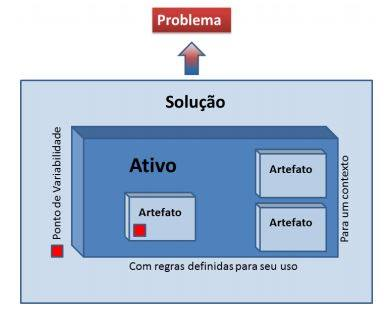
\includegraphics[width=0.5\textwidth]{images/ativo}
\centering
\caption{Ilustração de um ativo de software}
\label{Rotulo}
\end{figure}

  Ou seja, um ativo de software reutilizável é o conjunto que compõe a solução de um determinado problema, sendo composto por diferentes artefatos, que podem ser tanto códigos fontes, quanto documentação de projeto, ferramentas adotadas, entre outros artefatos.
 

    A OMG  utiliza três pontos-chave para descrever os ativos reutilizáveis, que apresentam-se como: Granularidade, Variabilidade e Articulação. A seguir descrevemos a definição de cada um destes.
    
 \begin{itemize}
    \item Granularidade: descreve a quantidade de problemas específicos ou soluções alternativas um pacote de artefatos pode resolver. Ativos mais simples, podem compreender um único problema bem definido. Porém com o aumento da complexidade do ativo em conjunto com o aumento de seu tamanho, a sua capacidade de resoluções de problemas aumenta junto a sua granularidade.
    \item Variabilidade: condiz com a capacidade do ativo fornecer variabilidade. Ou seja a possibilidade de alteração de suas caracteristicas, a OMG exibe as caracteristicas de variabilidade de um ativo por meio de um conjunto formado por quatro tipos:
    \begin{itemize}
         \item \textbf{Ativos caixa-preta:} a sua implementação interna não é conhecida e não pode ser alterada, por exemplo, componentes binários.
        \item \textbf{Ativos caixa-branca:} a sua implementação interna é conhecida e podem ser alterada, por exemplo, códigos fonte.
        \item \textbf{Ativos caixa-clara:} a sua implementação é conhecida, mas não podem ser modificados, por exemplo, documentação, modelos, fragmentos de código.
        \item \textbf{Ativos caixa-cinza:} a sua implementação é conhecida, porém apenas determinados subconjuntos de artefatos podem ser modificados, por exemplo, serviços disponibilizados, que em geral, permitem manipulação por meio de parâmetros.
    \end{itemize}
    
    \item Articulação: condiz com a capacidade do ativo de prover a solução do problema. Um ativo mais completo, constituído por exemplo de documentação, código fonte e testes que fornecem uma solução, possui um alto nível de articulação. 

\end{itemize}

    A biblioteca \textit{Hidra} aborda especificamente a segunda forma de armazenamento de ativos reutilizáveis de software.

\subsection{Ativos de Sotware}

    O RAS é descrito em duas principais categorias, o núcleo RAS e seus Perfis. O núcleo representa os elementos fundamentais para a especificação de uma ativo, e os perfis descrevem extensões desses elementos fundamentais. O perfil de uma ativo não altera a definição semântica de um elemento descrito no núcleo. O núcleo RAS não é instaciavel, assim como uma classe abstrata, portanto um ativo deve possui um perfil particular, esse perfil pode estender o núcleo RAS, ou estender um outro perfil como mostrado na figura a seguir.


\begin{figure}[H]
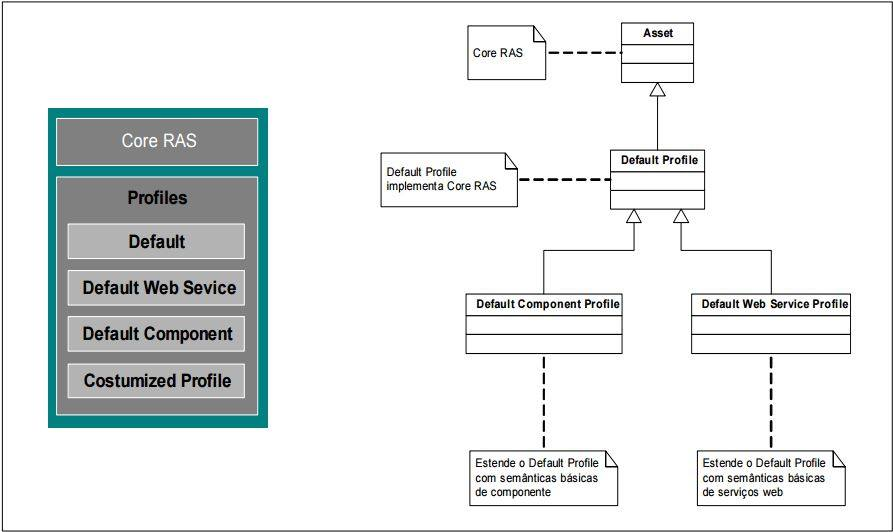
\includegraphics[width=0.8\textwidth]{images/estruturaAsset}
\centering
\caption{Estrutura de um Ativo de Softawe \cite{dissertacaoHenriqueFaria2005}}
\label{Rotulo}
\end{figure}

Um ativo de software é composto pela sua Classificação \textit{(Classification)}, Solução \textit{(Solution)}, Utilização \textit{(Usage)}, e pelo seu Perfil \textit{(Profile)}. Caso esteja relacionado a outros ativos também possuirá (Related Assets). A descrição de cada atributo é informada a seguir:

\begin{itemize}
    \item Classificação \textit{(Classification)}: : um conjunto de descritores que são usados para fazer a classificação do ativo, como descrever os contextos nos quais a reutilização do ativo é relevante.
     \item Solução \textit{(Solution)}: contém as descrições de um ou mais artefatos que fazem parte do ativo.
     \item Utilização \textit{(Soltuion)}: contém as regras para a instalação, customização e uso do ativo, ou seja, possui as instruções correspondentes a cada artefato que o ativo possui e um contexto de referência.
     \item Ativos Relacionados \textit{(Related Assets)}: condiz com as descrições dos relacionamentos existentes entre os ativos.
     \item Perfil \textit{(Profile)}: representa o perfil do ativo.
\end{itemize}
\begin{figure}[H]
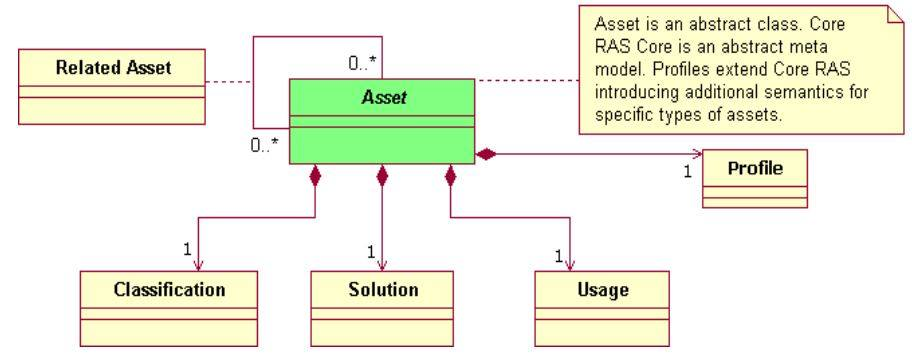
\includegraphics[width=0.8\textwidth]{images/modeloAsset}
\centering
\caption{ Estrutura de um ativo de Software (OMG, 2005)}
\label{Rotulo}
\end{figure}

\subsection{Considerações Finais}
    Nesta seção apresentamos as principais definições e orientações do modelo RAS utilizado como fonte de informação para desenvolvimento deste trabalho. Um dos aspectos abordados pela biblioteca Hidra é a validação, aceitação e persistência, em repositórios de ativos de software, condizentes com o padrão RAS descrito nesta seção.




% \makebox[\width]{Fonte: baseado em \citeonline[p.~4]{fulano}.}}
%     \label{interface}